\section{Virtual Presence and Telerobotics}
\label{intro:virtual_presence}

Man has always dreamt of being able to be present in more than
one place at the same time.
\\
In Hindu Mythology all the gods had multiple avatars, which
allowed them to exist in multiple domains simultaneously and to
serve the purpose of representing the original in different
places. In this way, gods could accomplished more useful work
at the same time. 
\\
This dream has always been one of the aims to achieve for 
researchers and industries. With the advent of Internet and
advanced computer and electronic technologies, we can get a
step closer to obtain presence in more than one place
at a time.
\\
What we need is the equivalent of a body in the remote environment,
with which we can move around, perform the proper actions through,
and observe with. By combining elements of Internet and
telerobotics it is possible to transparently immerse users into
navigable real remote worlds and to make such systems accessible
from any networked computer in the world. In essence, we obtain
\textit{Virtual Presence}.
\\
Virtual Presence removes the barriers of distance and offers a
reasonable facsimile of instantaneous travel to anywhere on earth
from any networked computer.
In Virtual Presence we have a telerobot which provides a form
(a physical avatar) that can be moved round in a remote space.
A telerobot is a robot that accepts instructions from a distance,
generally from a trained human operator. The human operator thus
performs live actions in a distant environment and through sensors
can gauge the consequences.
\\
The telerobot is hence equipped with a web-camera, laser scanning and
others type of sensors (see chapter \ref{intro:3morduc} for \morduc{}
concrete example). All these devices are used to provide the
necessary feedback for an effective feel of the remote domain.
\\
More formally, telerobotic is based on two main concepts, referred to
as \textit{teleoperation} and \textit{telepresence}.
\\
Teleoperation means `doing work at a distance', although `work' may
mean almost anything. The term `distance' is also vague: it can refer
to a physical distance, where the operator is separated from the robot
by a large distance, but it can also refer to a change in scale, where
for example in robotic surgery a surgeon may use micro-manipulator
technology to conduct surgery on a microscopic level.
\\
Telepresence means `feeling like you are somewhere else'.
Thus a user, sitting at a remote computer far away from the target
domain, can comfortably roam about, observe and even command
specific action to be performed in the vicinity of the telerobot.
\\
There are many jobs which a human could perform better than a robot, but
for some reasons humans either do not want to or can not perform it.
The job may be too dangerous, for example exploring inside a volcano;
other jobs must instead be executed in location physically inaccessible.
For example, exploring another planet, inspecting areas with very high
level of radiations, cleaning the inside of a long pipe or performing
laparoscopic surgery.
\\
Looking at these new perspectives robots are going to be more complex
than factories ones, built and programmed to accomplish few repetitive
tasks. Different kind of operations are not easy
to automate, and nowadays it is hard to develop autonomous robots, so
it is necessary to drive them by teleoperation and virtual reality.
\\
Looking back in history, some of our most influential technologies
- such as the telescope,
telephone, and television - were developed to provide knowledge
at a distance. Telerobotic systems date back to the need for handling
radioactive materials in the 1940s, and in the 1950's they were developed
to facilitate action at a distance. Remote controlled robot are now
being applied to exploration, bomb disposal, and surgery.
\\
Specialists use telerobots to actively explore environments such
as Mars and Chernobyl, while military personnel increasingly employ
reconnaissance drones and telerobotic missiles.
In the summer of 1997, the film Titanic included scenes with undersea
telerobots and NASA's Mars Sojourner telerobot successfully
completed a mission on Mars.
\begin{figure}
  \begin{center}
    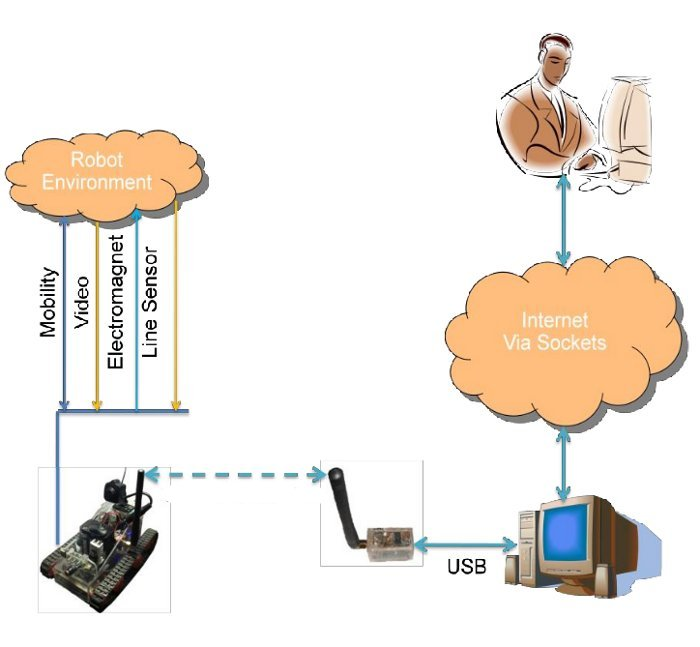
\includegraphics[width=270pt]{img/user_robot_inter.jpg}
    \caption{Generic Interaction human-robot through Internet}
    \label{fig:user_robot_inter}
  \end{center}
\end{figure}
\\
The Internet dramatically extends our scope and reach, since we can simply
teleguide the robot from any part of the world. The bidirectional
structure of the Internet offers furthermore a new means for actions:
through one communication channel telerobotic device can send data
collected by its sensors to the operator, in order to fulfil the
illusion of being in the remote place and to have a robust feedback;
on the other channel the operator can send the proper commands to
be performed by the robot. Illustration \ref{fig:user_robot_inter}
gives a graphical example.
